

\documentclass{article}
\usepackage[french]{babel}
\usepackage[letterpaper,top=2cm,bottom=2cm,left=3cm,right=3cm,marginparwidth=1.75cm]{geometry}
\usepackage{amsmath}
\usepackage{graphicx}
\usepackage{enumitem}
\usepackage{subfig}
\usepackage{float}

\usepackage[colorlinks=true, allcolors=blue]{hyperref}

\title{Projet 4 IA: Apprentissage par Renforcement}
\author{Berthion Antoine - 566199}

\begin{document}


\maketitle

\section{Introduction}
\label{sec:introduction}

\noindent Ce rapport a pour objectif de discuter des algorithmes de \textbf{value-iteration} et de \textbf{q-learning} dans le cadre des techniques de \textit{reinforcement learning}. Nous analyserons les algorithmes implémentés et examinerons les différents résultats obtenus en fonction des variations des paramètres propres à chaque algorithme. Par ailleurs, nous aborderons également l’impact de la nature aléatoire de l’environnement, qui ne correspond pas à un environnement déterministe.

\vspace{-2em} % Rapprocher la figure intro du texte intro

\begin{figure}[h]
    \centering
    \subfloat[Heatmap pour Value-Iteration]{%
        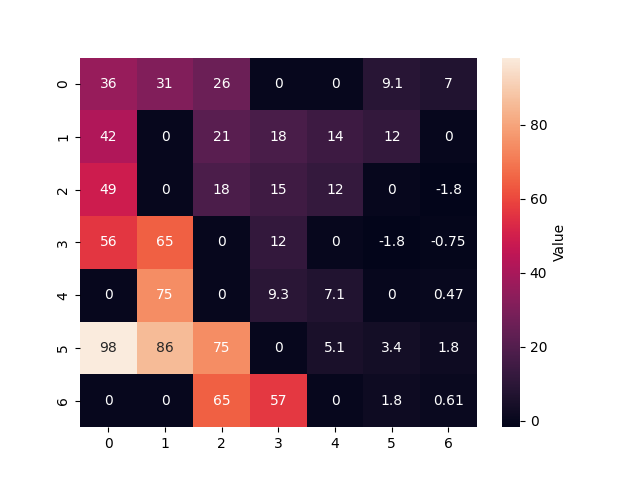
\includegraphics[width=0.45\textwidth]{src/intro1.png}
    }\hfill
    \subfloat[Heatmap pour Qvalues avec actions optimales]{%
        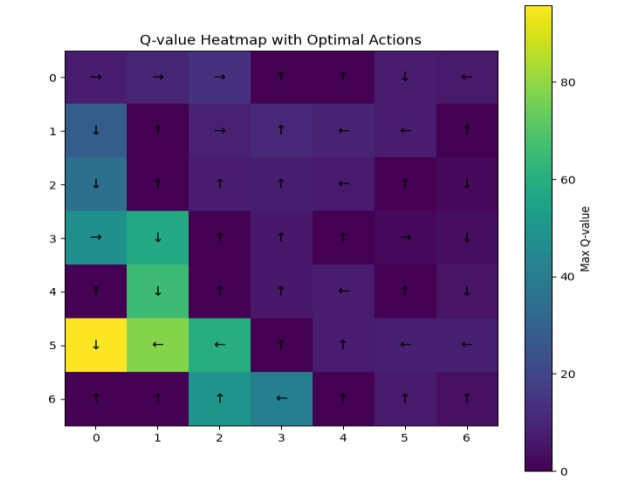
\includegraphics[width=0.45\textwidth]{src/intro2.png}
    }
    \caption{Résolution du problème de l'énoncé}
    \label{fig:intro}
\end{figure}

\vspace{-1em} % Rapprocher la figure intro du texte experimentations

\section{Expérimentations}
\label{sec:experimentations}

\noindent Dans cette section, nous menons une série d'expériences sur les algorithmes de \textbf{value-iteration} et de \textbf{q-learning}. Nous explorons l’impact de différentes configurations de paramètres sur les résultats obtenus. Les résultats de ces expériences seront analysés et discutés dans la section \ref{sec:discussion} de ce rapport.

\subsection{Expériences sur l'algorithme \textit{Value-Iteration}}

\noindent Nous allons générer la \textit{heatmap} correspondant au labyrinthe décrit dans l'énoncé, en entraînant successivement notre agent avec 10, 20, 30, puis 40 itérations de l'algorithme. \\

\noindent Le paramètre $\gamma=0.9$ (\textit{discount factor}) est fixé, afin d'indiquer à l'agent que les sorties doivent être atteintes aussi rapidement que possible pour maximiser le score. Par ailleurs, la composante aléatoire a été fixée pour chacune des quatre expériences, garantissant ainsi des résultats cohérents entre elles. Enfin, la fonction de récompense reste inchangée : elle attribue 10 points pour la sortie en $(3, 0)$, 100 points pour la sortie en $(0, 6)$, et -1 point pour toutes les autres cases. \\

\noindent Les résultats de nos expériences sont présentés ci-dessous, dans la figure \ref{fig:heatmap_v_iteration}.

\begin{figure}[H]
    \centering
    \subfloat[Heatmap (Value-Iteration), \textbf{10 itérations}]{%
        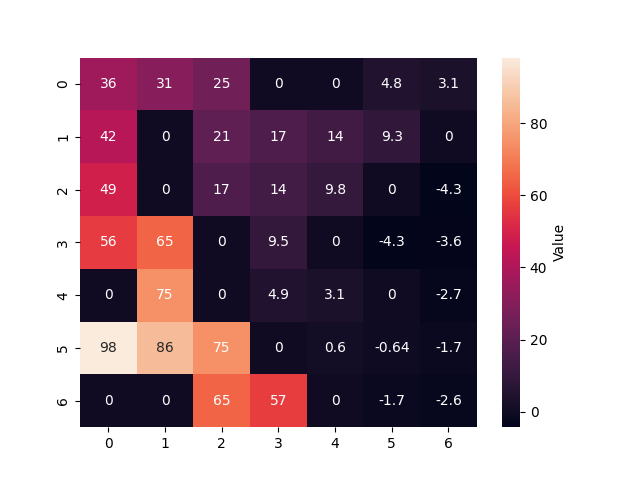
\includegraphics[width=0.45\textwidth]{src/value_iteration/10.png}
    }\hfill
    \subfloat[Heatmap (Value-Iteration), \textbf{20 itérations}]{%
        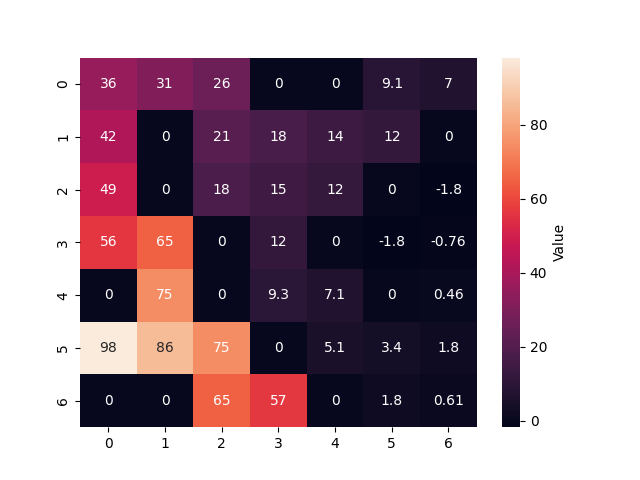
\includegraphics[width=0.45\textwidth]{src/value_iteration/20.png}
    }\\[-1.3em] % Saut de ligne pour la deuxième rangée
    \subfloat[Heatmap (Value-Iteration), \textbf{30 itérations}]{%
        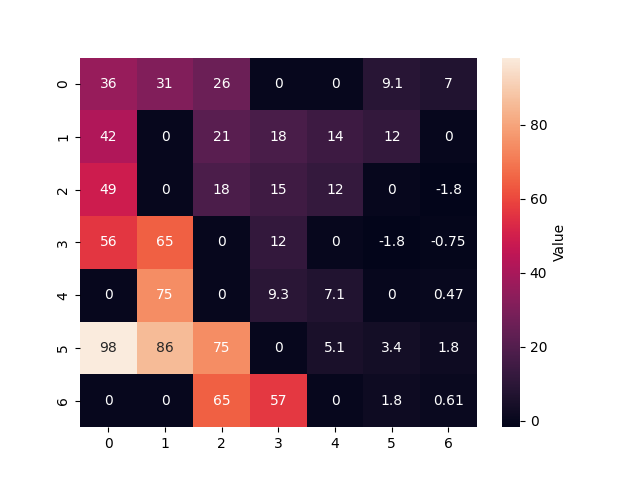
\includegraphics[width=0.45\textwidth]{src/value_iteration/30.png}
    }\hfill
    \subfloat[Heatmap (Value-Iteration), \textbf{40 itérations}]{%
        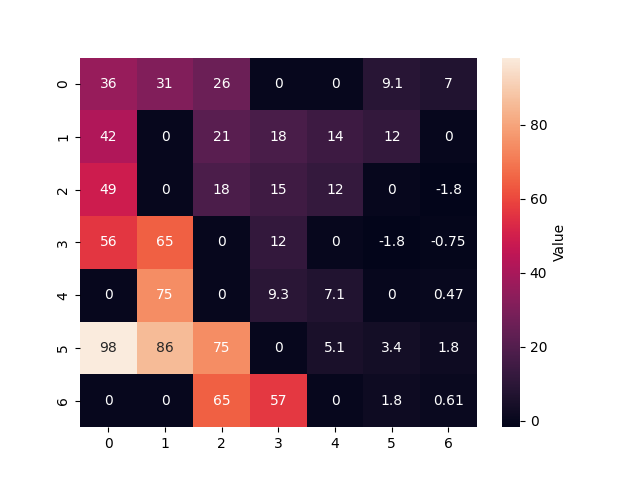
\includegraphics[width=0.45\textwidth]{src/value_iteration/40.png}
    }
    \caption{Heatmap Value-Iteration pour le labyrinthe de l'énoncé (10, 20, 30, 40 itérations)}
    \label{fig:heatmap_v_iteration}
\end{figure}

\subsection{Expériences sur l'algorithme \textit{QLearning}}

\subsubsection{Algorithme $\varepsilon$-greedy}
\label{subsubsec:egreedy}

\noindent Dans un premier temps, nous expérimenterons avec l'algorithme $\epsilon$-greedy. Nous tracerons un graphique représentant le score obtenu à chaque complétion du labyrinthe, c'est-à-dire la somme des récompenses accumulées par l'agent. Ce graphique sera accompagné d'une \textit{heatmap} indiquant la fréquence de visite des différentes positions dans le labyrinthe. L'expérience consistera à faire varier le paramètre $\epsilon$, tout en maintenant le paramètre \textit{c} (bonus d'exploration) fixé à 0. De plus, nous fixerons le \textit{learning rate} $\alpha$ à 0.1 et le \textit{discount factor} $\gamma$ à 0.9.

\begin{figure}[H]
    \centering
    {%
        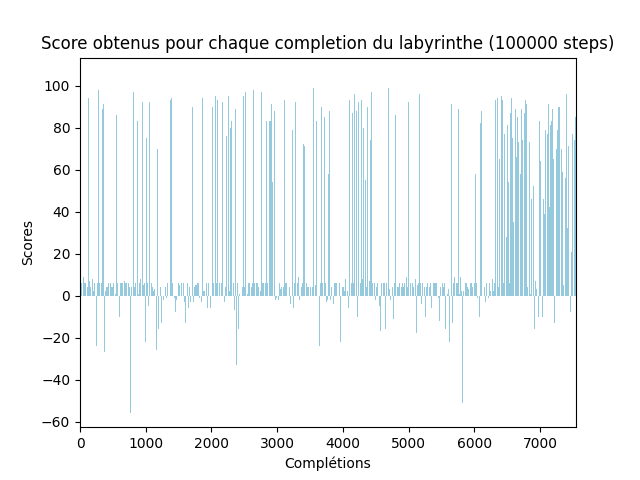
\includegraphics[width=0.45\textwidth]{src/qlearning/greedy/greedy02.png}
    }\hfill
    {%
        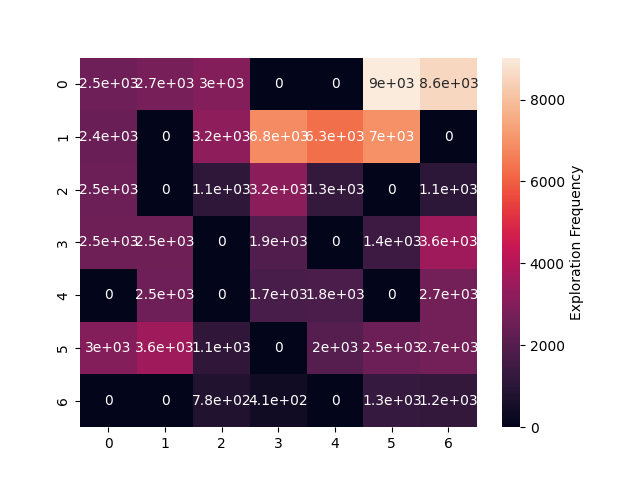
\includegraphics[width=0.45\textwidth]{src/qlearning/greedy/greedy02heatmap.png}
    }
    \caption{Qlearning (100 000 steps) $|$ $\varepsilon$ = 0.2}
    \label{fig:egreedy02}
\end{figure}

\begin{figure}[H]
    \centering
    {%
        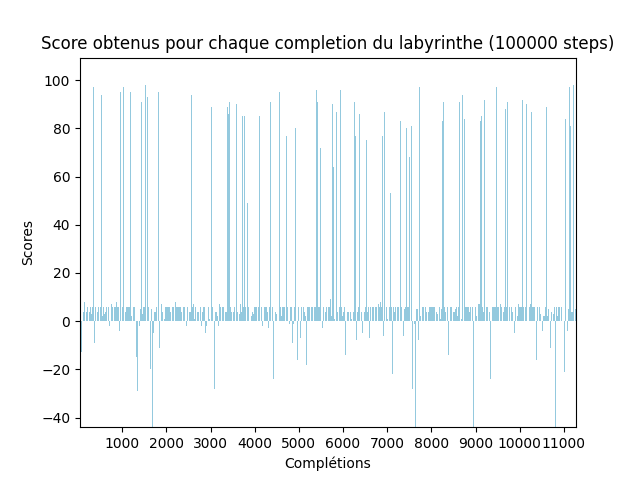
\includegraphics[width=0.45\textwidth]{src/qlearning/greedy/greedy01.png}
    }\hfill
    {%
        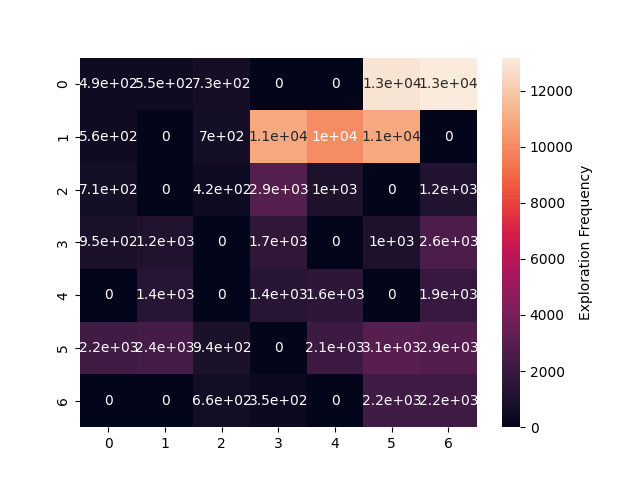
\includegraphics[width=0.45\textwidth]{src/qlearning/greedy/greedy01heatmap.png}
    }
    \caption{Qlearning (100 000 steps) $|$ $\varepsilon$ = 0.1}
    \label{fig:egreedy01}
\end{figure}

\begin{figure}[H]
    \centering
    {%
        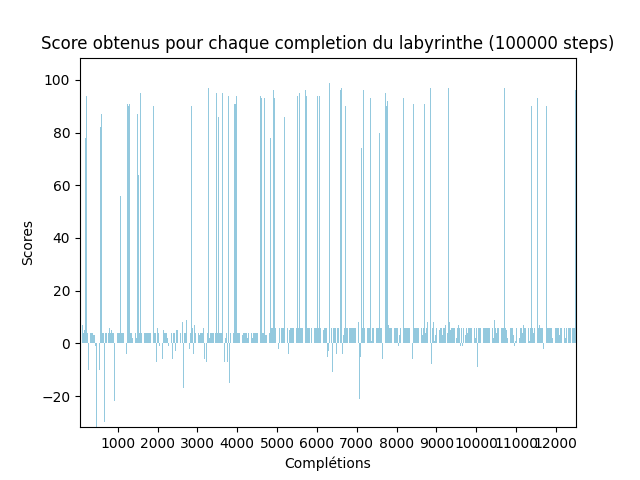
\includegraphics[width=0.45\textwidth]{src/qlearning/greedy/greedy001.png}
    }\hfill
    {%
        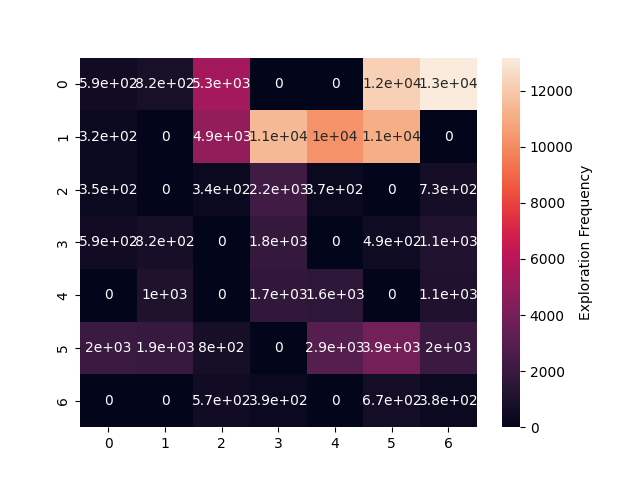
\includegraphics[width=0.45\textwidth]{src/qlearning/greedy/greedy001heatmap.png}
    }
    \caption{Qlearning (100 000 steps) $|$ $\varepsilon$ = 0.01}
    \label{fig:egreedy001}
\end{figure}

\subsubsection{Algorithme avec Bonus d'exploration}
\label{subsubsec:exploitation}

\noindent Dans un second temps, nous expérimenterons avec la stratégie du bonus d'exploration. Pour ce faire, nous fixerons le paramètre $\varepsilon$ à 0, puis ferons varier le paramètre $c$. Les autres paramètres de l'expérience précédente restent fixés.

\begin{figure}[H]
    \centering
    {%
        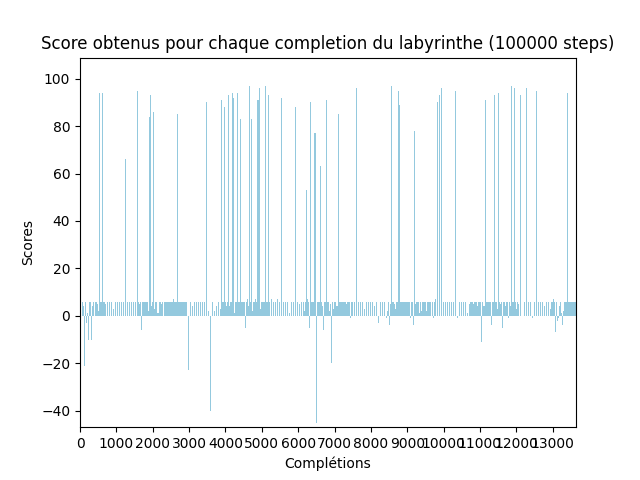
\includegraphics[width=0.45\textwidth]{src/qlearning/bonus/bonus1.png}
    }\hfill
    {%
        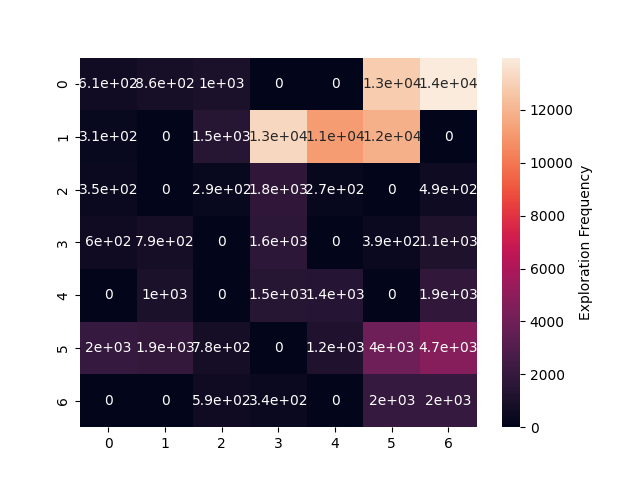
\includegraphics[width=0.45\textwidth]{src/qlearning/bonus/bonus1heatmap.png}
    }
    \caption{Qlearning (100 000 steps) $|$ $c$ = 1}
    \label{fig:bonus1}
\end{figure}

\begin{figure}[H]
    \centering
    {%
        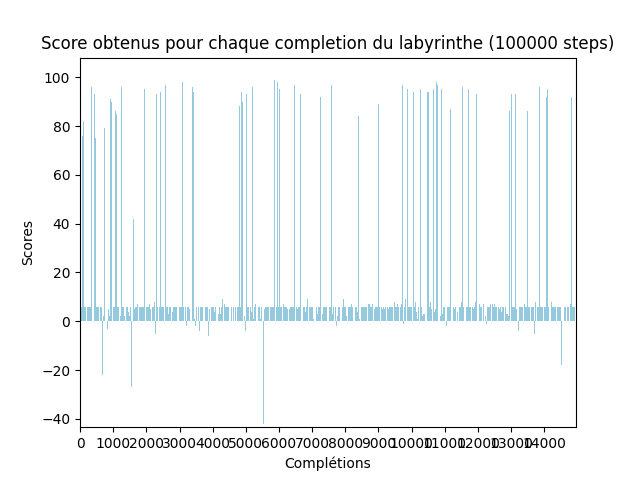
\includegraphics[width=0.45\textwidth]{src/qlearning/bonus/bonus10.png}
    }\hfill
    {%
        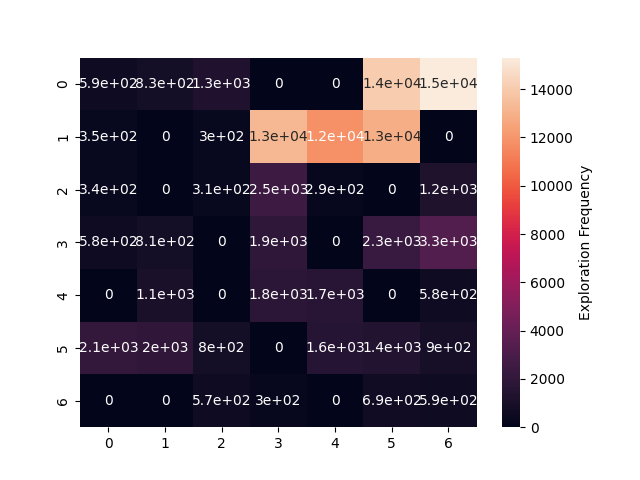
\includegraphics[width=0.45\textwidth]{src/qlearning/bonus/bonus10heatmap.png}
    }
    \caption{Qlearning (100 000 steps) $|$ $c$ = 10}
    \label{fig:bonus10}
\end{figure}

\begin{figure}[H]
    \centering
    {%
        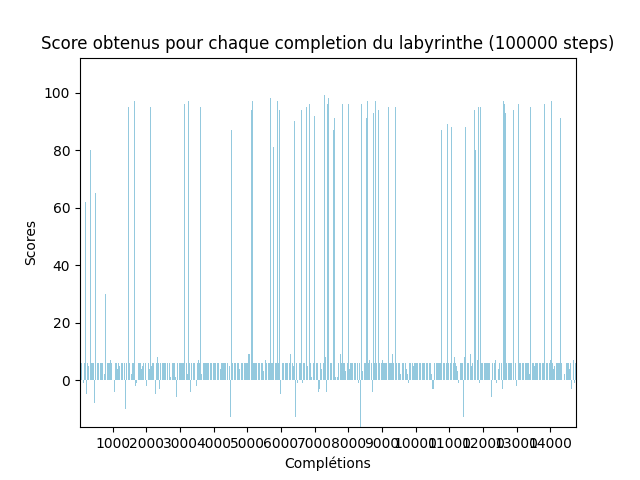
\includegraphics[width=0.45\textwidth]{src/qlearning/bonus/bonus100.png}
    }\hfill
    {%
        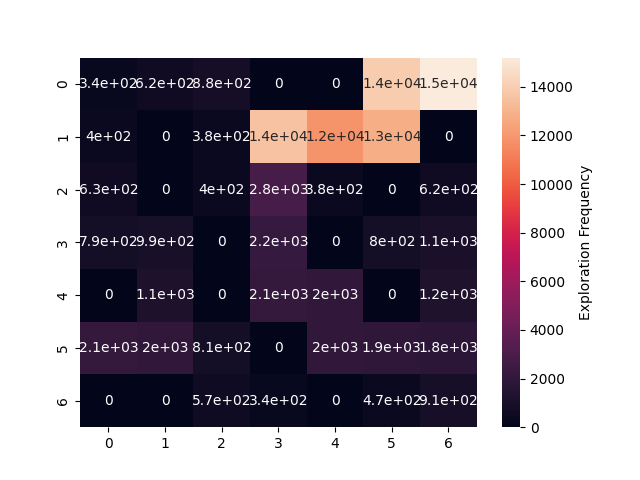
\includegraphics[width=0.45\textwidth]{src/qlearning/bonus/bonus100heatmap.png}
    }
    \caption{Qlearning (100 000 steps) $|$ $c$ = 100}
    \label{fig:bonus100}
\end{figure}

\begin{figure}[H]
    \centering
    {%
        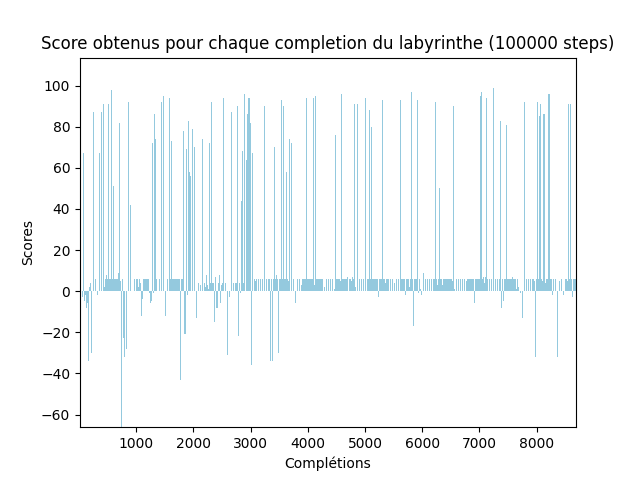
\includegraphics[width=0.45\textwidth]{src/qlearning/bonus/bonus1000.png}
    }\hfill
    {%
        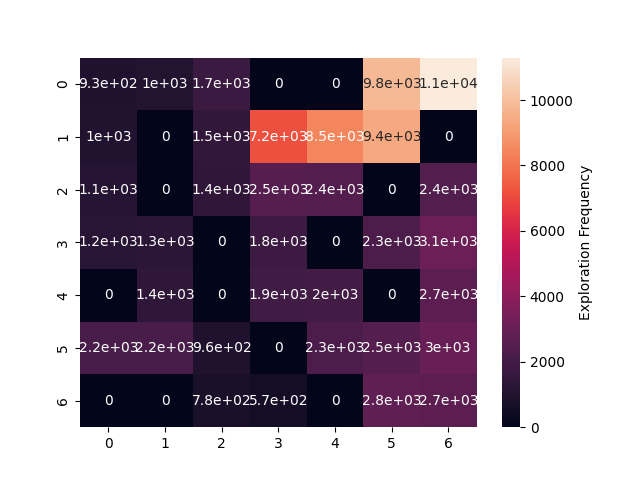
\includegraphics[width=0.45\textwidth]{src/qlearning/bonus/bonus1000heatmap.png}
    }
    \caption{Qlearning (100 000 steps) $|$ $c$ = 1000}
    \label{fig:bonus1000}
\end{figure}


\subsubsection{Sensibilité des paramètres}

\noindent Dans cette sous-section, nous nous concentrerons sur les effets de la modification de certains paramètres d'entraînement, afin de pouvoir étudier leur sensibilité. Nous mesurerons la récompense moyenne obtenue par l'agent pour une action, tout au long des \textit{steps}. La configuration par défaut utilisée est la suivante :

\begin{itemize}
    \item Le \textit{discount-factor} $\gamma = 0.9$
    \item Le \textit{learning rate} $\alpha = 0.1$
    \item Le \textit{bonus d'exploration} $c = 100$
    \item La \textit{variable d'exploration} $\varepsilon = 0$
\end{itemize}

\noindent Nous étudierons les variations des paramètres suivants : $\gamma$, $\alpha$ et $p$ (la probabilité que l'environnement soit corrompu et téléporte l'agent aléatoirement). Les résultats, présentés ci-dessous, sont issus d'un entraînement réalisé sur 10 000 \textit{steps}. L'expérience sera répétée 20 fois, afin de garantir la meilleure précision possible et d'éliminer, autant que possible, le facteur non déterministe.

\begin{figure}[H]
    \centering
    % Ligne supérieure (une image centrée)
    \subfloat[Sensibilité du paramètre $p$]{%
        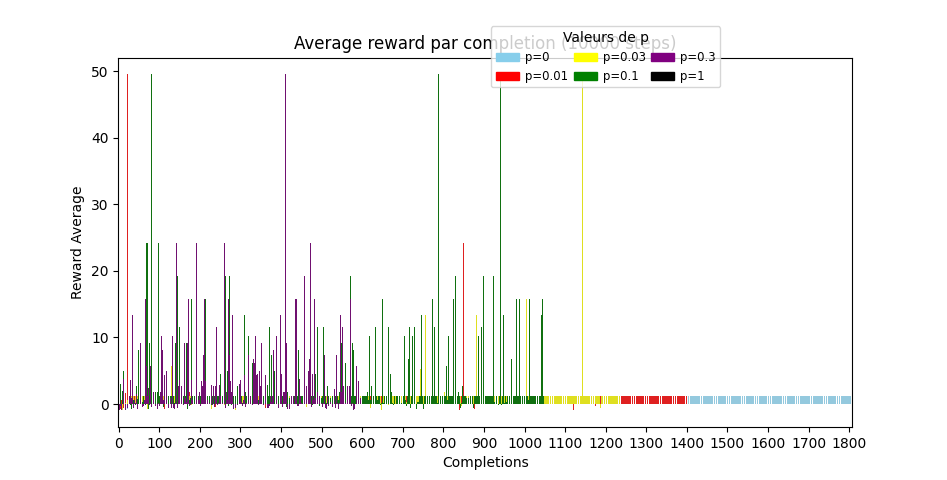
\includegraphics[width=0.6\textwidth]{src/parameters/p_sensibility.png}
        \label{fig:p_sensibility}
    } \\
    % Ligne inférieure (deux images côte à côte)
    \subfloat[Sensibilité du paramètre $\alpha$]{%
        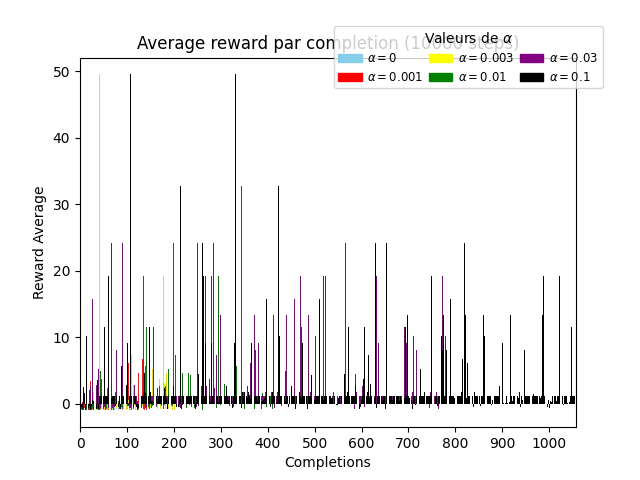
\includegraphics[width=0.45\textwidth]{src/parameters/alpha_sensibility.png}
        \label{fig:alpha_sensibility}
    }
    \hfill
    \subfloat[Sensibilité du paramètre $\gamma$]{%
        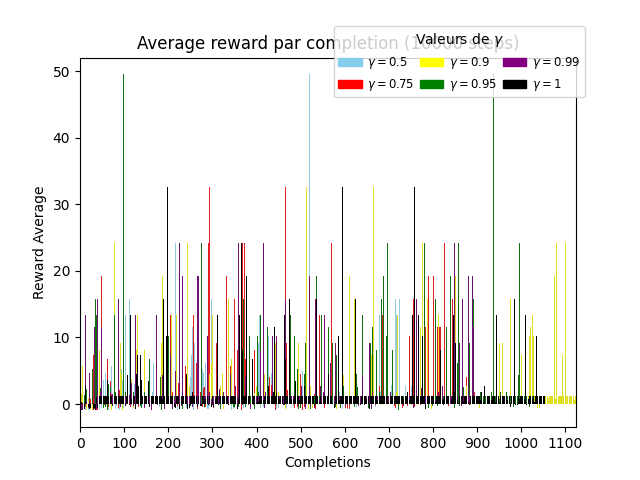
\includegraphics[width=0.45\textwidth]{src/parameters/gamma_sensibility.png}
        \label{fig:gamma_sensibility}
    }
    \caption{Analyse de la sensibilité des paramètres $\gamma$, $\alpha$, et $p$}
    \label{fig:sensibility_analysis}
\end{figure}

\noindent Ainsi s’achèvent nos expériences. Dans la section \ref{sec:discussion}, nous discuterons de leur interprétation et répondrons aux questions liées aux méthodes d’implémentation et d’utilisation des algorithmes de \textit{value-iteration} et de \textit{q-learning}.

\section{Discussion des résultats expérimentaux}
\label{sec:discussion}

\noindent Discutons dès à présent des résultats obtenus dans la section précédente (section \ref{sec:experimentations}). \\

\noindent Pour commencer, intéressons-nous à la figure \ref{fig:p_sensibility}. Nous savons que l'environnement est non-déterministe, ce qui influence considérablement l'efficacité des algorithmes. Dans un environnement totalement aléatoire, l'algorithme devient pratiquement inutile, car il ne serait pas capable de prendre des décisions ayant un impact réel. À l'inverse, si l'environnement est complètement déterministe, le Q-learning sera particulièrement efficace, car il pourra toujours choisir la meilleure option disponible, ce qui entraîne des valeurs convergeant vers l'optimalité.

\noindent Cependant, il est important de noter que la nature aléatoire de l'environnement peut parfois être bénéfique. En effet, elle pousse l'agent à se retrouver dans des états qu'il n'aurait normalement pas explorés. Cela peut être avantageux, en particulier lorsque le bonus d'exploration ou le paramètre epsilon sont trop bas. Dans ce cas, l'agent pourrait hésiter à explorer suffisamment, se limitant ainsi à des récompenses petites mais sûres. Cela ne constitue pas toujours la meilleure stratégie à long terme, car l'agent pourrait passer à côté de meilleures opportunités si l'exploration est trop restreinte.

\noindent Il apparaît dans nos résultats qu'un paramètre $p$ relativement bas garantit des résultats satisfaisants. Toutefois, nous observons qu'en augmentant cette probabilité, les scores obtenus sont plus élevés, mais avec une moyenne généralement plus basse. Cela peut s'expliquer par le fait que certaines corruptions ont un effet très positif, rapprochant l'agent de la sortie valant le maximum de points. Il est juste de dire que la probabilité de non-déterminisme se reflète dans les Q-values, quelle que soit la méthode utilisée. Cependant, les algorithmes restent conscients de cette probabilité et intègrent ces perturbations dans leurs calculs, de manière pondérée par la valeur de $p$. En conséquence, ils parviennent, en moyenne, à rester relativement précis et à obtenir des scores moyens positifs. \\

\noindent Dans un second temps, nous discuterons de la nature des algorithmes \textit{$\varepsilon$-greedy} et \textit{d'exploration}. Ces deux algorithmes sont fondamentalement opposés : l'un cherche à obtenir les meilleures récompenses disponibles de manière sûre, tandis que l'autre privilégie des choix plus risqués. En effet, l'algorithme d'exploration peut offrir des récompenses plus élevées pour les états moins visités, mais cela implique parfois de prendre des décisions sous-optimales, tout en offrant la possibilité de faire de meilleurs choix à long terme.

\noindent Observons les graphiques présentés dans les sous-sections \ref{subsubsec:egreedy} et \ref{subsubsec:exploitation}. On constate que l'algorithme exploitant produit des résultats beaucoup plus constants. Comme prévu, les heatmaps associées montrent des zones principalement colorées sur les cases menant à la sortie la plus sûre, mais qui rapportent le moins de points. Les autres cases restent peu explorées. En revanche, l'algorithme explorateur génère des résultats plus variables, mais avec des extrêmes plus marqués. Concrètement, il peut obtenir de très mauvais résultats, mais aussi, dans certains cas, des performances bien supérieures.

\noindent Ainsi, si notre objectif est de converger rapidement vers une solution satisfaisante, l'algorithme \textit{$\varepsilon$-greedy} est à privilégier. En revanche, si nous souhaitons explorer et nous assurer qu'il n'existe pas de meilleure solution, l'algorithme d'exploration s'avère être un meilleur choix. \\

\noindent Abordons maintenant brièvement le facteur d'apprentissage $\alpha$, ou \textit{learning rate}. Plus ce paramètre est élevé, plus les valeurs récentes auront un poids important par rapport aux anciennes. En d'autres termes, les résultats les plus récents seront privilégiés. Il est particulièrement utile d'avoir un facteur d'apprentissage élevé lorsque l'algorithme est explorateur, car les événements très positifs sont moins fréquents, et il est donc crucial de leur accorder plus de poids. En revanche, lorsque l'on utilise un algorithme exploitant, il n'est pas nécessaire de mettre autant l'accent sur chaque état, car les récompenses sont plus prévisibles et stables.

\noindent Expérimentalement, comme illustré dans la figure \ref{fig:alpha_sensibility}, nous avons observé que la valeur optimale de $\alpha$ semble se situer autour de $0.1$. Des valeurs extrêmes, telles que $0$, conduisent à des résultats absurdes, notamment un apprentissage inexistant dans ce cas particulier. \\

\noindent Enfin, abordons le \textit{discount factor}, $\gamma$. Ce paramètre permet de moduler l'importance des récompenses futures en les réduisant au fur et à mesure du temps. En d'autres termes, plus $\gamma$ est faible, plus les récompenses sont dévaluées à mesure qu'elles deviennent lointaines. L'idée initiale pourrait être de fixer $\gamma$ aussi bas que possible, mais cela comporterait des risques. En effet, si la valeur de $\gamma$ est trop faible, l'agent pourrait être incité à rechercher un état terminal le plus rapidement possible, sans se soucier de la qualité de la récompense. Il est donc important de trouver un compromis, en choisissant un $\gamma$ intermédiaire entre 0 et 1. D'après nos expériences, la valeur optimale de $\gamma$ semble se situer autour de $0.95$, comme le montre la figure \ref{fig:gamma_sensibility}.

\section{Utilisation des LLM}

\noindent Dans cette courte partie, nous discuterons de l'utilisation des LLM dans le cadre du projet. Aucun LLM n'a été utilisé pour l'aspect implémentation ainsi que la compréhension du projet. Cependant, ce rapport à été corrigé du point de vue de la syntaxe et de la grammaire par DeepL ainsi qu'un modèle GPT. Notons tout de même qu'aucune des informations du rapport n'a été produite par une autre personne que l'auteur.

\end{document}
